\documentclass[10pt]{article}
\usepackage{graphicx}
\usepackage{siunitx}
\usepackage{listings}
\usepackage{color}
\usepackage{mathptmx}
\usepackage[export]{adjustbox}
\usepackage{float}
\usepackage{amsmath}
\usepackage[a4paper,bindingoffset=0.2in,%
            left=1in,right=1in,top=1in,bottom=1in,%
            footskip=.25in]{geometry}
\title{EE314 Digital Electronics Laboratory Term Project Proposal Report \\* FPGA Based Oscilloscope}
\date{2018\\ May}
\author{Ekin Yılmaz - 2094738 Nail Tosun - 2094563\\ Electric and Electronic Engineering Departmant, METU}
\begin{document}
\maketitle
\section*{Introduction}
In this project a simple FPGA based oscilloscope which can visualize a given single frequency input signal from a signal generator with different waveforms on VGA screen and which can also measure the given parameters in Table 1 is aimed to be designed. Iteration limit here is what determines the resolution. Since the limit is given as 250, using 20mV steps a maximum of 0 to 5 Volts range can be scanned via these steps. 

\begin{table}[H]
\centering
\caption{The required measurements that the designed oscilloscope can achieve}
\label{my-label}
\begin{tabular}{ccc}
Parameter & \begin{tabular}[c]{@{}c@{}}Max-Min\\   Values\end{tabular} & Resolution \\
Frequency & DC – 20kHz                                                 & 10 Hz      \\
Vpp       & 0 to 5 Volts                                               & 20 mV      \\
Vrms      & 0 to 5 Volts                                               & 20 mV      \\
Voffset   & 0 to 5 Volts                                               & 20 mV     
\end{tabular}
\end{table}
\section*{Working Prinsiple of Design}
For this purpose a system which consists of a ADC measuring module to quantize the signal, a data storage module where the transmitted quantized data is stored, a computation module that performs the required measurements and calculations to determine frequency, peak-to-peak voltage, waveform, rms voltage, and offset voltage and finally a VGA display module where the visualization of the results is realized, is designed. Related block diagram of the overall system can be seen in Figure 1. In addition to these modules, there will be also a mode selection input which decides whether the oscilloscope will measure in AC coupling mode or DC coupling mode. According to the decision made, entire signal will be visualized for DC mode or DC value will be subtracted first then the signal will demonstrated in AC mode. This mode selection part will be realised via switches on the FPGA board. Finally, there must be also adjustable time/div, volt/div and autoscale option too. Those arrangements will be done by using push buttons on the board.

\begin{figure}[H]
  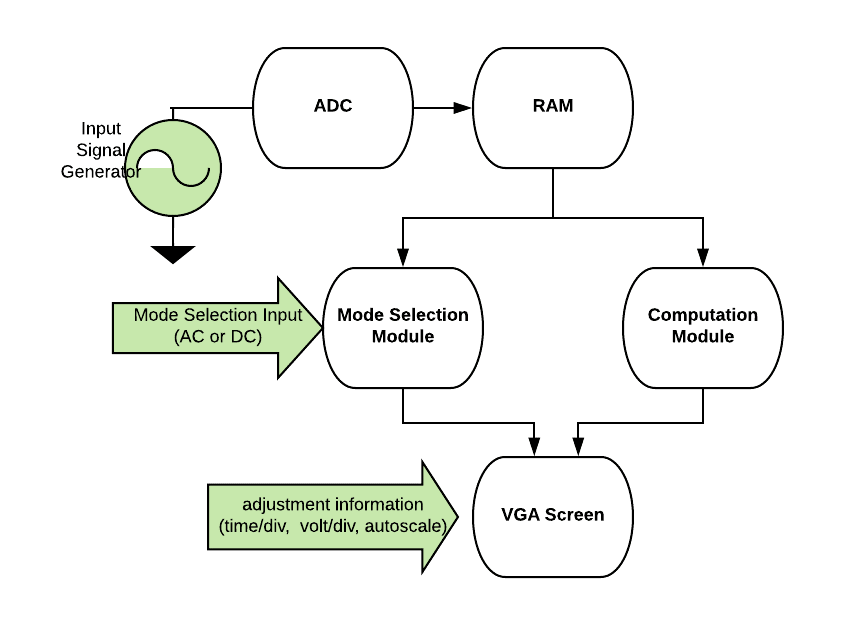
\includegraphics[scale=0.7, center]{blockdiagram}
  \caption{Block diagram of the overall system}
  \label{fig:zero}
\end{figure}
\section*{Equipment}
VGA connector, VGA display screen, De1-SoC FPGA development board.
Mainly the VGA outputs and embedded ADC of the board will be used in this project. Input signals will be applied from the ADC header and the output will be taken from the VGA output of the development board for visualization.
\section*{Rms voltage measurement unit}
Starting the design, an RMS voltage measurement module is designed first since it will also be a crucial part of AC DC selection module too.

Discrete RMS formula is following;
\[V_{rms}=\sqrt{\frac{1}{N}\sum\limits_{i=0}^{N-1}V_i^2}\]
Then we firstly took square every serial in values. This module HDL code is following;

Then we sum squares of serial in values after to one period and divide the period $N$ for mean value of squares. (Frequency of the signal is an    \textit{input} for this module). HDL code is following;
\begin{lstlisting}[language=Verilog, caption=Averaging module]
module rms_finder(clk, freq, average, serial_in);
input clk;
input [11:0] serial_in;
input [31:0] freq;
output reg [31:0] average;
integer index,N,dum_index,sum; 
initial
begin
period = 0;
sum <= 0;
N <= 0;
index <= 0;
average <= 0;
dum_index <= 1;
end
always @(posedge clk)
begin
	//N=f_sampling/freq //input and sampling frequency determines the N
	N = 8; //for testing
	if (index<N)
		begin
		sum <= sum + serial_in;
		index <= index+1;
		end
	else if(index==N)
	begin
	dum_index <= dum_index + 1;
	average <= sum/(N*dum_index);
	index <= index +1;
	dum_index <= dum_index + 1;
	end
	else index <= 0;
end
endmodule

\end{lstlisting}

Then we write another module that simple take square root of the input. HDL code of this module is following;

\begin{lstlisting}[language=Verilog, caption=Square-root module]
module m(clk, mean_input, rms);
input clk;
input [11:0] mean_input;
output reg [11:0] rms;
reg [11:0]temp=1;

always@(posedge clk)
begin
	if((temp*temp)>=mean_input)
		rms<=temp;
   else
      temp<=temp+1;
  end
endmodule
\end{lstlisting}
\section*{Simulation Results}
\begin{figure}[H]
  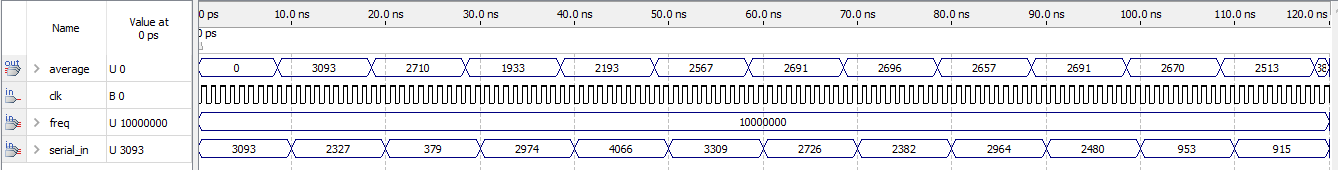
\includegraphics[scale=0.5, center]{Mean_finder}
  \caption{Simulation results of mean-finder}
  \label{fig:zero}
\end{figure}


\begin{figure}[H]
  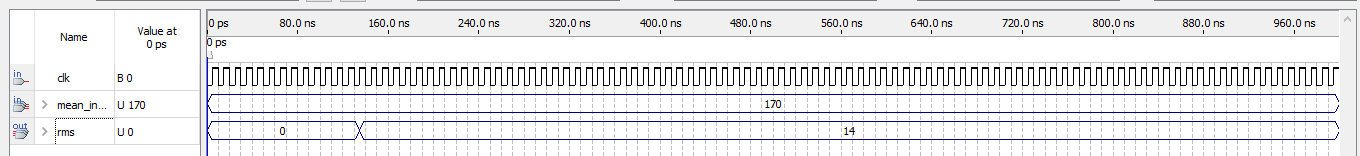
\includegraphics[scale=0.5, center]{Rms_out}
  \caption{Simulation results of square root module}
  \label{fig:zero}
\end{figure}
\end{document}
